%%% File encoding: UTF-8
%% äöüÄÖÜß  <-- no German Umlauts here? Use an UTF-8 compatible editor!

%%% Magic comments for setting the correct parameters in compatible IDEs
% !TeX encoding = utf8
% !TeX program = pdflatex 
% !TeX spellcheck = en_US
% !BIB program = biber

\documentclass[master,english]{hgbthesis}
% Permissible options in [..]: 
%   Type of work: diploma, master (default), bachelor, internship 
%   Main language: german, english (default)
%%%----------------------------------------------------------

\RequirePackage[utf8]{inputenc}		% Remove when using lualatex or xelatex entfernen!
\usepackage[titletoc]{appendix}
\usepackage[acronym]{glossaries}
\usepackage{enumitem}
\usepackage{adjustbox}
\usepackage{array}
\usepackage{minted}

\newcolumntype{R}[2]{%
    >{\adjustbox{angle=#1,lap=\width-(#2)}\bgroup}%
    l%
    <{\egroup}%
}
\newcommand*\rot{\multicolumn{1}{R{45}{1em}}}% no optional argument here, please!

\newcommand{\norm}[1]{\left\lVert#1\right\rVert}


\graphicspath{{images/}}    % location of images and graphics
\logofile{dhbw-logo}				% logo file = images/logo.pdf (use \logofile{} for no logo)
\bibliography{references}  	% name of bibliography file (references.bib)

\setcounter{tocdepth}{4}
\setcounter{secnumdepth}{4}

%%%----------------------------------------------------------
% Title page entries
%%%----------------------------------------------------------

%%% Entries for ALL types of work: --------------------------
\title{Design and implementation of a computer aided ergotherapy framework}
\author{Georg Grab}
\programname{Computer Science}
\placeofstudy{Stuttgart}
\dateofsubmission{2018}{06}{04}	% {YYYY}{MM}{DD}

\advisor{Dirk Reichardt, Prof. Dr.} 

\makeglossaries

\loadglsentries{other/acronym}
\loadglsentries{other/glossary}

\begin{document}
\frontmatter

\maketitle
\tableofcontents
\listoffigures
\printglossary[type=\acronymtype,title=Acronyms]
\printglossary[title=Glossary]

\include{front/abstract}

%%%----------------------------------------------------------
\mainmatter          			% main part (arabic page numbers)
%%%----------------------------------------------------------
\chapter{Introduction}
\label{sec:introduction}
\section{Problem description}
In 2016, approximately 60.000 German residents have been hospitalized due to hand or wrist injuries \cite{DeStatisHandInjuries}. The inpatient treatment of such injuries is often followed by a lengthy recovery phase in which ergotherapeutic treatment occurs in order to further aid recovery. As ergo therapy sessions are usually held in one-on-one sessions, this results in a significant time and resource investment both by the patient and the treating clinic. Additionally, the sessions themselves are often described by patients as boring and unmotivating, citing their repetitive nature.

Ergo therapists of the Katharinenhospital Stuttgart are currently researching alternative treatment methodologies that could constitute an improvement to all three of these fundamental problems. The aim of the research is to introduce various gamification aspects to the recovery sessions. The patients should be enabled to perform repetitive parts of the recovery exercises at home by means of successfully executing them while controlling video games. This methodology of executing prevention and rehabilitation measures is an active and well known field of research commonly referred to as Exergames \cite{RehaCareExergames}. In a more general sense, games that are designed with a second primary purpose (apart from entertainment) are referred to as serious games \cite{SeriousGamesBook}. 

\section{Project Scope}
\label{sec:scope}
The scope of this student research project is to design and provide implementations for a software solution acting as an underlying framework on which the Exergames can be executed. The framework should be capable of meeting the determined requirements as outlined in section \ref{sec:reqanalysis} either directly through the provided implementation, or, if some requirements cannot be fulfilled with the reference implementation, by way of easy extensibility. The framework should also contain a user facing component where relevant measurements and game configurations can be made and from which the games are executed. Additionally, the framework should contain various tools that will make it easier for future developers to develop and debug subcomponents.

\section{Requirements Analysis}
\label{sec:reqanalysis}
Outsourcing recovery exercises into a space where no direct therapeutic supervision is available generates a series of challenges that have to be identified and overcome before successfully integrating Exergames in the recovery sessions. 

\subsection{Functional Requirements}
\label{sec:frs}
In a software development context, the challenges a system has to solve in order to become useful to the stakeholders are referred to as functional requirements \cite{SystemRequirementsArmyFR}.  The most notable functional requirements are outlined as follows.

\subsubsection{Domain Virtualization}
\label{sec:freq:domain-virtualization}
In order for Exergames to fundamentally function, they require an accurate, real-time virtualized representation of the problem domain. For example, in order to develop Exergames for treating hand injuries, a virtual representation of the hand must be available. For the domain of upper extremities, several hardware devices exist that are capable of providing the virtualized representations. Notable examples are the Leap Motion Device by Leap Motion, Inc.\footnote{\url{https://www.leapmotion.com}}, and Microsofts Handpose technology for the Kinect Device\footnote{\url{http://research.microsoft.com/en-us/projects/handpose/}}. Both devices, normally used in the context of \gls{VR} and \gls{AR}, are capable of producing the virtual representation by employing a variety of hardware sensors.

\subsubsection{Exercise Classification}
\label{sec:exercise-classification}
The most important capability of an Exergame is to correctly classify whether a recovery exercise has been executed. In the domain of hand and wrist injury recovery, a recovery exercise may for example be the spreading of the thumb, where the remaining fingers of the hand remain closed. Other examples for recovery exercises have been outlined by \cite{StudiArbeitVolzBaumotte}. The result of the exercise classification can then be used as a gameplay element in the Exergame. For example, if a thumb spread exercise as described above has been executed well enough, a \emph{Space Invaders-like} Exergame could trigger the space ship to shoot.

\subsubsection{Patient Adaptibility}
One-on-one therapy sessions in ergo therapy are required because of the large variety of different hand injuries, each requiring a different set of recovery exercises. Additionally, the classification logic (see \ref{sec:exercise-classification}) for the recovery exercises themselves have to be adaptable to how far the patient has progressed so far in recovery. For example, if the patient is progressing well in recovery, the relevant exercise has to be increased in difficulty in order for the treatment to remain effective.

\subsubsection{Monitorability}
\label{sec:req:monitorability}
The ergo therapist has to be able to view monitoring information related to the patients playing activity. Most fundamentally, the therapist should be able to view the number of times and total duration of Exergames played in order to verify if the agreed upon exercise volume has been completed. Additionally, specific information that aid the ergo therapist in assessing the recovery progress of the patient should be available. If the therapist determines that the current exercise has to be adapted in some way, or for exchanging other kinds of information with the patient, such as providing hints or agreeing on the next physical appointment date, this should be possible through an integrated messaging platform. Furthermore, the monitoring information should be able accessible through a web-based interface.

\subsubsection{Gameplay and Frontend}
\label{sec:gameplay}
Finally, the system should provide a frontend component, from which the actual games are executed and configured, and where display components relevant for resolving other software requirements can be found.

\subsection{Non-Functional Requirements}
In addition to the functional requirements, the following \glspl{NFR} have to be considered while designing and implementing the system. \glspl{NFR} are global requirements that are not directly related to function, but refer to the development or operational costs of the system, such as performance, reliability, and maintainability \cite{chung2012non}.

\subsubsection{Modularization}
\label{sec:nfr:modularization}
On a technical level, the program logic responsible for classifying if an exercise has been completed (see \ref{sec:exercise-classification}) should be separated from the actual Exergames logic (see \ref{sec:gameplay}). This would pose the advantage of introducing a modular aspect to the system, as both exercise classifiers and games could be exchanged, both keeping the patients engaged in the platform by allowing them to practice their assigned exercise using a variety of games, and greatly simplifying the work of future developers, as they will be enabled to develop games for the platform without any prior knowledge of exercise classification, and vice versa.

\subsubsection{Performance}
\label{sec:nfr:performance}
Performance is a critical \gls{NFR} for the system. All data coming from the device providing the relevant domain virtualization has to be ingested, preprocessed, and classified in real time. If this is not the case, the patient will experience a significant lag between the performed exercise and the feedback of the Exergames, quickly resulting in frustration. Additionally, the execution of the Exergames themselves should be performant enough so that the gameplay experience isn't negatively obstructed. 

\subsubsection{Availability}
\label{sec:nfr:availability}
From the therapist point of view, it is critical that the platform is capable of running without an active network connection. This results in the technical restriction that all network connections made by the platform must be both optional and fault tolerant. This requirement originates from the assumption of the therapists that the system will not always be used in contexts where an internet connection is readily available.


\subsubsection{Ease of deployment}
\label{sec:nfr:deployment}
The system should ultimately be primarily executed on a patient provided device. As such, deployment of the application should be easy, and robust with respect to a multitude of possible, previously unknown target environments.

\subsubsection{Extensibility}
\label{sec:nfr:extensibility}
As the system is acting primarily as an underlying framework on which other developers should build upon in the future, it should be written in a way that allows for easy extensibility. It should especially be written in a computer programming language that is well known to the potential target developer audience, so minimum prior knowledge is required before starting development with the project. Additionally, the framework should be future proof: it should be simple to exchange subcomponents with more modern equivalents in the future. For example, it should be simple to add support for more modern hardware devices providing domain virtualization, or more modern graphics libraries for developing the Exergames in the future.


\section{Outline and structure}
Section \ref{sec:introduction} gave a general overview of the project motivation, scope, and method. Additionally, the project requirements gathered in various in person meetings with the stakeholding therapists were outlined.

Section \ref{sec:relatedwork} presents prior relevant work on the subject of computer aided ergotherapy and puts this work into context. The following section will introduce the relevant technologies and theoretical foundations used in the implementation phase of the project.

The main part of this paper is constituted by section \ref{sec:impl}, where possible project architectures are presented, the project reference implementation is detailed and architecture and technology choices are justified. The work concludes with the recommended next steps in developing the system (section \ref{sec:future}), and a critical conclusion (section \ref{sec:conclusion}).

% fully featured web platform, because modern web technologies allow it, GUI Application does not fit the requirements, and separating main work into server thread is, while potentially more performant, both potentially insecure and unnecessarily complex.
\chapter{Related Work}
\label{sec:relatedwork}

The general feasibility of using devices such as the Leap Motion for different usecases than their primary intended purpose in the entertainment industry, specifically using them for clinical purposes, has already been shown by various research.

In 2014, researchers from the University of California have successfully developed an Exergame version of the popular smartphone game \emph{Fruit Ninja}, utilizing the Leap Motion Device for domain virtualization \cite{khademi2014free}. The researches have shown that the Game could purposefully be used for stroke rehabilitation by showing that a strong correlation exists between the achieved score while playing the \emph{Fruit Ninja} game, and standard clinical assessment scores.

The feasibility of using the Leap Motion device for developing Exergames specifically in the context of the Web browser have been shown by \cite{DigitizingHandRehabilitation}. In the work, the authors showed the general feasibility of web based digital hand rehabilitation by implementing and evaluating Web based Exergames on a prototypical level. In an earlier work, the same researchers have shown that the Leap Motion device is capable of delivering a virtualized hand representation of sufficient accuracy for tracking the patients rehabilitation progress \cite{AnalyzingHandTherapySuccess}.

In a research project completed in 2017, students of the DHBW Stuttgart initially collaborated with ergo therapists of the Katharinenhostpital Stuttgart in order to determine requirements for a web based handtherapy system that would be mature enough to be deployed at hospitals at a bigger scale \cite{StudiArbeitVolzBaumotte}. In the project, some preliminary system requirements have been identified, and recommendations for the architecture and implementation of the system have been given. In addition, some of the recovery exercises that the system should be able to assimilate have been documented.
\\\\
This work follows up on the previous research by providing an architecture and reference implementation for a mature, holistic hand therapy system that is ready to be used by ergo therapists and their patients as an accompaniment for hand and wrist injury rehabilitation.
\include{chapters/3_technologies_methods}
\chapter{Framework Implementation}
\label{sec:impl}
\section{Architecture Decision}
\subsection{Available Alternatives}
Based on the requirements outlined in section \ref{sec:reqanalysis}, which have been gathered and derived in various in-person meetings with the stakeholding therapists, multiple technologies for implementing the system seem feasible. The alternatives considered at the beginning of this project are outlined as follows.

\subsubsection{Fully featured Web Application}
\label{sec:alt:fully-featured-web-app}
One technological possibility would be to implement the core system framework as a fully featured Web Application. All requirements would be implemented using web technologies. Most notably, data ingestion, preprocessing, classification, and monitoring would have to be accomplished entirely in the context of a web browser. The system would be self-sufficient in this configuration, without reliance on any external systems, though an external server component for sending the monitoring information is conceivable (see requirement \ref{sec:req:monitorability}).

This configuration is very favorable in terms of deployment and extensibility, as every component is consistently written in Javascript, the standardized programming language of the web. Likewise, as functionality is not distributed over multiple systems, the deployment of the systems only requires a web browser\footnote{The installation of relevant hardware device drivers on the target device is also required for the system to function, but as the same is true for all other alternatives, this is not considered under the ease of deployment aspect.}.

However, for this configuration to be feasible, it is required that the domain virtualization device contains an API to the Web Browser. Also, the Javascript programming language is sometimes critizied for its relatively poor performance when compared to programming languages with compilers capable of producing native code. This is owed in large parts to the dynamically typed and interpreted nature of the language. Some benchmarks show that Javascript is up to ten times slower in terms of runtime performance compared to C++ when running computationally expensive tasks \cite{BenchmarksGame}. The question of whether Javascript is performant enough to tackle the task at hand has to be clarified before this alternative can be considered feasible.
\subsubsection{Web Application with local server component}
\label{sec:alt:thin-web-app}
The two main disadvantages of the fully featured Web Application, the need for a Web API of the virtualization device and the performance considerations, could be mitigated by moving the computationally expensive logic in a locally running server component, and interfacing the two components by using an asynchronous communication specifications such as WebSockets or XmlHttpRequest. As the code running in the server component is running with Operating System permissions, it could directly interface with the hardware device. Additionally, all logic concerned with working with the virtualization device data could be implemented in native code, resulting in high performance.

This approach in turn poses the disadvantage that a lot of additional complexity is introduced into the system. The system would no longer be implemented in a single programming language. Additionally, the system would no longer be easy to deploy, as compiled binary packages would have to be provided and thoroughly tested for each desired target Operating System.
\subsubsection{Web Application with remote server component (backend)}
\label{sec:alt:thin-remote-web-app}
Following up on the design outlined in section \ref{sec:alt:thin-web-app}, the system could also be designed with a remote server component instead of a locally running server. This would have the advantage of all device data being available
at one centralized location, where very elaborate analytics could be performed. As all alternatives outlined in this section will eventually require a backend component for accumulating monitoring information for the therapist to view and inspect, this approach initially seems to reduce complexity.

However, the virtualized domain data would again have to be ingested by the Web Application, in a similar fashion to the alternative outlined in \ref{sec:alt:fully-featured-web-app}, as no local application is available to handle the connection to the hardware device. Furthermore, all virtualization device data would have to be sent over the network connection of the end device, potentially resulting in high latency, and possibly full system outage if the end device fails to establish an internet connection.
\subsubsection{Desktop Application}
\label{sec:alt:desktop-app}
Finally, the system could be designed without relying on Web technologies altogether, and be instead implemented as a traditional Desktop Application.

\begin{table}[h]\footnotesize
\caption{Comparison of implementation alternatives based on estimated requirement fulfillment}
\label{alt:table-requirement-comparison}
\renewcommand{\arraystretch}{1.3}
\begin{tabular}{l|cccccc}
    &
    \rot{Functional Reqs.} &
    \rot{Modularization} &
    \rot{Performance} &
    \rot{Availability} &
    \rot{Deployment} &
    \rot{Extensibility}
        \\ \hline
    Desktop App (\ref{sec:alt:desktop-app})               &   & X & X & X &   &   \\ 
    Web thin client (\ref{sec:alt:thin-web-app})          & X & X &   &   & X & X \\ 
    Web local client (\ref{sec:alt:thin-remote-web-app})  & X & X & X & X &   &   \\
    Web fat client (\ref{sec:alt:fully-featured-web-app}) & X & X & ? & X & X & X \\ \hline
\end{tabular}
\normalsize
\end{table}
\subsection{Elected Alternative}
Table \ref{alt:table-requirement-comparison} gives an overview over the likely requirement fulfillment of the discussed implementation alternatives. 
\\
The Desktop Application is the only proposed architecture incapable of intrinsically meeting the functional requirements: as the therapists plan on viewing and evaluating the platform monitoring data from a Web based interface, a separate application would need to be developed for that sole purpose. Regarding the \glspl{NFR}, Performance and Modularization can be fulfilled easily, as statically typed, modern programming languages that compile to platform-native code can be employed. In addition, the system could be designed in such a way that meets the Availability requirement. However, as the architecture cannot fulfill all Functional Requirements, and additionally lacks the \glspl{NFR} of Deployment (platform dependant binary must be provided) and Extensibility (future developers will likely need to learn a new programming language), this alternative is ruled out as a potential platform architecture.
\\\\
While the Web based thin client outlined in section \ref{sec:alt:thin-remote-web-app} is capable of implementing all functional requirements, the architecture is ruled out as it is relying on a remote server for basic functionality, resulting in a failure to meet the Availability \gls{NFR}. Additionally, even if a network connection is available, there are serious considerations to be made regarding network latency. The latency aspect imposes a performance dependency on the quality of the users internet connection, resulting in at least unreliable performance.
\\\\
The Web based client backed up by a local webserver as outlined in section \ref{sec:alt:thin-web-app} solves the problems of the Web based thin client regarding Availability and Performance, however, the ease of deployment aspect would be lost by the fact that a native platform binary is required for executing the application. Also extensibility is jeopardized, as a large amount of complexity is introduced into the system, most notably the fact that two separate programming languages or frameworks would be required for developing the system. While these tradeoffs would certainly not be critical, this choice of architecture is considered unfavorable for the time being.
\\\\
The fully featured Web Application has the theoretical capability to meet all functional requirements. Additionally, most non-fuctional requirements can be met by the architecture: the modern Javascript ecosystem allows for modularization and code splitting capabilities through the use of ES6 Modules. Furthermore, supersets of the language exist that provide support for static typing, such as Typescript. A static type system has the advantage that programming interfaces may be explicitly typed, so the program becomes easier to extend by developers not fully familiar with the program as a whole \cite{TypescriptUnderstanding}. It can be assumed that development on the Web platform is well known to the target developer audience, as it is a well established topic that is teached in most computer science related university courses. In addition, the architecture is easy deploy on the target end devices: in essence, all that is required from the end users is to navigate to a Website using a relatively recent Internet Browser. While this action initially seems to break the Availability requirement, modern Web Specifications, most notably the Service Worker Specification, allow for the application to still be available if the network connection is lost \cite{serviceworkersdraft}. The only non-functional requirement of the application that is in need for clarification is whether the architecture supports adequate performance for resolving the task at hand. However, several Web technologies are currently developed to mitigate this exact problem. Most notably, the widely adoped Web Workers specification essentially allows for developing multi threaded applications on the Web \cite{workerdraft}. Additionally, the WebAssembly specification has recently reached a mature state and is available in all major browsers. WebAssembly is a binary instruction format designed to be deployed on the web, allowing for web developers to develop code executing at near native speed while maintaining cross platform compatibility \cite{wasmdraft}.

Based on the considerations employed in this section, the fully featured Web Application is chosen as the system architecture, as it seems to support implementation of all imposed requirements.

\section{System Architecture}

\begin{figure}[h]
    \centering
    \includegraphics[width=10cm]{highlevelarch}
    \caption{High Level Architecture Overview}
    \label{fig:high-level-architecture}
\end{figure}
A high level overview of the resulting architecture is outlined in Figure \ref{fig:high-level-architecture}. High level architecture components are prepresented as rectangles, relations between them are displayed as arrows. An \emph{includes} relationship is illustrated by nested rectangles. The architecture closely follows the state management pattern recommended by Vuex. 

The Frontend, illustrated by a single rectangle in this case, communicates with the Application State by signifying desired state changes (for example, the ticking of a checkbox) by commiting mutations. At the same time, the Frontend components declare a dependency on relevant parts of the state. If these parts of the state update, Vuex automatically rerenders the dependant Frontend components in order to reflect the changes.

The Application State itself contains, apart from the state of the Frontend Components, references to the other subcomponents of the application, namely references to a component facilitating persistence, configuration information for data preprocessors and classifiers, and finally a reference to the device facade component, which facilitates access to the device driver implementation. These components are further elaborated in the following sections. 

\subsection{Frontend}
\label{sec:impl:frontend}
\begin{figure}[h]
    \centering
    \includegraphics[width=14cm]{frontend}
    \caption{Frontend: Detailed Subcomponent Overview}
    \label{fig:frontend-overview}
\end{figure}

As Figure \ref{fig:frontend-overview} illustrates, the frontend is divided in a number of subcomponents, each responsible for fulfilling a specific purpose.

\subsubsection{Debug Interface}
The Debug Interface is responsible for diagnosing problems if the connection to the motion tracking device cannot be established, and for providing development tooling. It is thus mainly responsible for contributing towards the Extensibility \gls{NFR} (section \ref{sec:nfr:extensibility}). The Interface consists of three subcomponents.

\paragraph*{Raw Device Logger}

The Raw Device Logger is a Frontend Component capable of displaying the raw device frames as they arrive. The component receives the incoming data stream, and formats it in order to be human readable. As new data arrives, the Component updates itself automatically, making it possible to inspect the incoming device data over time. The Component acts as a developer tool, allowing the developer to view live device data, and thus gain intuition over how the device data is structure and how it is changing over time.

\paragraph*{Graphical Device Logger}

Similarly, the Graphical Device Logger is acting on the incoming device data stream, but instead of formatting the raw data in a textual manner, it is interpreted graphically. Using the Three.JS library (\ref{sec:tech:threejs}), graphical hand and finger objects are created and displayed inside a 3-dimensional coordinate system.

\begin{figure}[ht]
    \centering
    \includegraphics[width=8cm]{graphical-hand-logger}
    \caption{The Graphical Hand Logger.}
    \label{fig:graphical-hand-logger}
\end{figure}

Figure \ref{fig:graphical-hand-logger} illustrates the graphical representation the component is able to produce for Leap Motion Device Data. The Component is able to display other device data as well, though only illustrations based on Leap Motion Device Data are implemented as part of this work. The Leap-Motion specific illustration is constructed by first projecting the interactionBox-relative positional device data (see section \ref{sec:tech:leap-domain-model}) in the THREE.js coordinate system by applying the formula

\begin{equation}
x_{proj} = proj_{min} + (proj_{max} - proj_{min}) * \dfrac{x_{leap} - iBox_{min}}{iBox_{max} - iBox_{min}}    
\end{equation}

to each dimension of relevant positional data, where $x_{proj}$ is the target position, $proj$ describes the bounds of the target projection, $x_{leap}$ is the positional data of the Leap Motion Device, and $iBox$ describes the bounds of the interactionBox. 

Afterwards, the palm is drawn by constructing a 2-dimensional disc, and sizing, positioning, and rotating it according to the transformed hand data. The fingers are drawn by constructing a 3-dimensional tube from each pointable object of the frame data. The tube is constructed from the skeletal tracking information of the pointable and interpolated using a Centripetal Catmull-Rom spline. This type of interpolating curve is widely used in the field of computer graphics because of several useful mathematical properties \cite{Yuksel2011}.

\paragraph*{Device Status Log}
The Device Status Log is the final debugging component of the framework. The Status Log portrays the state of the three main failure points of the application. The main failure points include the connection of the Javascript Device Driver to the Native Device Driver (see \ref{sec:tech:leap-hardware-driver}), the availability of the Native Device Driver, and the Physical availability of the hardware tracking device. The Framework is able to detect the state of all three of these failure conditions, and displays instructions to the user on how to mitigate these problems in case one or more failures occur.

\subsubsection{Hand Measurement}
The ergo therapist is required to measure angles between certain bones of the hand in order to determine how the patient is progressing in recovery \cite[sec. 4.1.6]{StudiArbeitVolzBaumotte}. The digitized ergo therapy system should be able to perform these measurements as well in order to reduce the manual workload of the therapist.

The reference implementation of the system includes a frontend component with the ability to take measurements of the angles between neighboring fingers. Other types of measurements are able to be integrated in the framework easily by using existing code structure and utility functions. The measurements are able to be averaged across a configurable timeframe in order to achieve more accurate results. The angle calculation itself is performed by applying the formula

%export const calculatePointableAngle = (
%  first: LeapPointable,
%  second: LeapPointable
%): number => {
%  const ab = first.direction
%    .map((el, idx) => el * second.direction[idx])
%    .reduce((p, c) => p + c, 0);
%  const normFirst = norm(first.direction);
%  const normSecond = norm(second.direction);
%  const theta = Math.acos(ab / (normFirst * normSecond));
%  return theta * 180 / Math.PI;
%};
\begin{equation}
angle = \arccos(\dfrac{\vec{p_1} * \vec{p_2}}{\norm{\vec{p_1}} * \norm{\vec{p_2}}}) * \dfrac{180}{\pi}
\end{equation}

to the directional vectors of neighboring fingers.

\subsubsection{Preprocessing and Classification Configuration}
The stream pre-processing and classification frameworks, outlined in further detail in sections \ref{sec:impl:preprocessing} and \ref{sec:impl:classify} respectively, require user configuration from the frontend. The available subcomponents that are available for each framework can be toggled on or off, and supplied with configuration that the subcomponent requires. Every change made in the Frontend configuration will automatically be propagated through the system, and will be available immediately.

\subsubsection{Game Listing}
The most integral part of the system is for the patient to be able to play games by means of performing the relevant recovery exercises as dictated by the therapist (see section \ref{sec:frs}). In order to implement this functionality in the system, the frontend has a component where the available Games are listed. For each available Game, a short title and description is shown. Furthermore, this component validates if the system is ready to execute the game (i.e., the motion tracking device is plugged in and functioning normally, and a classifier has been activated, as outlined in \ref{sec:impl:classify}). After the component has validated that the system is ready, a Play Button becomes available to the user. After the Play Button has been pressed, the component hands control to the Game Execution Framework (see section \ref{sec:impl:gameexec}).

\subsubsection{Hand Recorder}
\label{sec:impl:hand-recorder}
The Hand Recorder is a Frontend Component with the primary purpose to alleviate framework developers from having to physically connect a hand tracking device in order to develop preprocessors, classifiers, or games for the platform. The component allows to record series of device frames. Optionally, the recordings may be titled, and persisted in the Persistence Provider implementation (see section \ref{sec:impl:persist}). If a previously saved recording is activated using this component, the contained frames will be propagated in an endless loop through the framework as if they were coming from a physical device. Only one saved recording may be active at any given time. If a hand tracking device is already connected and functioning as expected, the data coming from the recording will be preferred. Furthermore, the user is able to download saved recordings, for example in order to reproduce bugs, or using them for illustration purposes in other parts of the system.

\subsection{Device Facade Interface}
The Device Facade Interface is the primary access point for frontend components that wish to work with motion tracking device data. The Interface, named after the well-known Facade pattern in Software Development \cite{Gamma:1995:DPE:186897}, decouples the Frontend Components both from the actual implementation of the Device Driver (see section \ref{sec:impl:driver}), as well as the actual data source (i.e., Recording, Physical, or potential future data sources).


Figure \ref{fig:device-facade-interface} shows an excerpt of the Interface. References to \gls{RX} streams representing Hand Tracking Data, Classification Data (see \ref{sec:impl:classify}), and the DeviceDriver implementation itself may be obtained. Additionally, the Facade may receive Configuration updates regarding the Data Preprocessing and Classification Frameworks from Frontend Components, which will subsequently be relayed into the Device Driver for further processing.
\begin{figure}
\begin{minted}{typescript}
export interface DeviceFacade {
    getHandTrackingData: (
      store: Store<RootState>
    ) => Observable<GenericHandTrackingData> | undefined;
    getClassificationStream: () => Observable<ClassificationData> | undefined;
    getDeviceDriver: () => DeviceDriver;
    updatePreProcessors: (x: PreProcessorConfig[]) => void;
    updateClassifier: (x: ClassifierConfig) => void;
    ...
}
\end{minted}
\caption{Device Facade Interface Definition (excerpt)}
\label{fig:device-facade-interface}
\end{figure}
The Interface is bound to the desired Implementation at compile time through dependency injection, and registered to the global application state on page load.

The System contains a reference implementation of the Device Facade Interface, named \emph{AllPurposeFacade}, though different implementations, for example a mock implementation for utilization in Unit Tests, are conceivable.
\subsection{Device Driver Interface}
\label{sec:impl:driver}
Components implementing the Device Driver Interface are primarily responsible for handling the connection to the physical device from the Web Context. In case of the Leap Motion Platform, such a connection is obtained by connecting to a local Websocket Server provided by the Leap Motion Hardware Device Driver \emph{leapd} (see section \ref{sec:tech:leap-hardware-driver}). Other potential Motion Tracking Devices, such as the Microsoft Kinect Platform, provide similar methods of accessing the Hardware Device from a Web Context \cite{KinectSDK}. New Device support can thus be added to the platform by means of adding a Device Driver Implementation, and optionally providing the parts of the Platform that depend on specific Device Data with the relevant device-specific implementations, for example providing rendering methods for the new Device to the Graphical Device Logger (see \ref{sec:impl:frontend}, par. \emph{Graphical Device Logger}).
\begin{figure}
\begin{minted}{typescript}
export interface DeviceDriver {
  deviceName: string;
  establishConnection: () => Observable<DeviceConnectionState>;
  getTrackingData: () => Observable<GenericHandTrackingData>;
  getClassificationData: () => Observable<ClassificationData> | undefined;
  enableClassification: (classifiers: string[]) => void;
  updatePreProcessors: (configs: PreProcessorConfig[]) => boolean;
  updateClassifier: (config: ClassifierConfig) => boolean;
  digest: (data: GenericHandTrackingData) => void;
  ...
}
\end{minted}
\caption{Device Driver Interface Definition (excerpt)}
\label{fig:device-driver-interface}
\end{figure}

Figure \ref{fig:device-driver-interface} illustrates the methods and properties that must be implemented by Device Drivers. The \texttt{deviceName} property must be defined on the implementing class. This property acts as a unique device identifier across the whole system. If device specific implementations are required for some parts of the system, they are resolved using this identifier. The method \texttt{establishConnection} is used to signal to the DeviceDriver that a connection should be established. This method is called on system start. The method must return a \gls{RX} Observable representing the connection state to the device driver over time. After \texttt{establishConnection} has been called, the DeviceDriver should automatically attempt to reconnect to the native device driver if the connection has been lost or could not be established initially, and update the Observable on each registered change of connectivity.

The \texttt{getTrackingData} method must return a \gls{RX} Observable that should emit the tracking data each time a new frame is received by the driver. The generic type of a device frame is named \texttt{GenericHandTrackingData}. The concrete implementations of the Interface may extend this type in order to explicitly type the data coming from the device. The methods \texttt{enableClassification}, \texttt{updatePreProcessors}, and \texttt{updateClassifier} are used to signal to the device driver that its internal Data Preprocessing and Classification pipelines should update. These subcomponents of the Device Driver are further explained in sections \ref{sec:impl:preprocessing} and \ref{sec:impl:classify}.

Finally, it is possible to inject arbitrary data into the Device Driver by means of calling the \texttt{digest} method. The Device Driver is responsible for processing the data coming through this method in the same way that real device data is processed. This enables testing of the Device Driver without requiring a physical hardware device, and furthermore provides the technical foundation for tooling such as the Hand Recorder (section \ref{sec:impl:hand-recorder})

As part of this work, two implementations of the Device Driver interface are provided: \texttt{LeapMotionDeviceDriver} and \texttt{ThreadedLeap2Driver}, both providing support for the Leap Motion Device. While the \texttt{LeapMotionDeviceDriver} only provides minimal support for the most basic functionality, the \texttt{ThreadedLeap2Driver} provides a full implementation of all required functionality. Additionally, this implementation is spawning a Web Worker (see section \ref{sec:tech-web-worker}) internally, so all data ingestion and preprocessing is performed in a separate thread, ensuring performant operation for the rest of the system.

\subsection{Persistence Framework}
\label{sec:impl:persist}
It can be argued that the User Experience of a complex software product improves significantly if it has the capability of persisting the User Configuration over subsequent visits. If this were not the case, the User would have to reenter any settings that have been made previously each time the application is restarted. In the context of Web Applications, various possibilities exist for persisting data, such as storing and loading the data from a Backend, saving the data using Browser Cookies, or using more recent Web Specifications such as Local Storage or IndexedDB.

All of these technologies have several advantages and disadvantages. In addition, it does not actually matter for the end user \emph{how} the data is stored in most scenarios, as long as it is stored in the first place. The system thus provides a \texttt{PersistenceProvider} Interface, which contains methods representing create, read, update, and delete functionality for persisted records. The System is shipped with one ready to use implementation of the \texttt{PersistenceProvider} interface, which is named \texttt{IndexedDBPersistenceProvider}, using IndexedDB as the concrete persistence technology. The \texttt{PersistenceProvider} is available to the whole application, as it is registered in the global application store (see figure \ref{fig:high-level-architecture}).


\subsection{Stream pre-processing framework}
\label{sec:impl:preprocessing}
As mentioned briefly in section \ref{sec:impl:frontend}, the user has the option to configure various data pre-processors. The goal of pre-processors may be to provide more accurate data to subsequent system components, or reduce workload by stopping unnecessary data from further propagating through the system. The configuration, which pre-processors have been activated by the user and how they are configured, is supplied to the device facade, and subsequently, the device driver implementation, on each change. In the case of pre-processors, the configuration consists of an array of configuration objects, in turn consisting of a unique pre-processor identifier, and an array of pre-processor specific configuration options. The Device Driver implementation should now call the provided entrypoint to pre-processing framework, named \texttt{PreProcessingResolver}, with the received configuration. The \texttt{PreProcessingResolver} internally looks up the pre-processing identifier in the \texttt{PreProcessingRegistry}, where the identifier is resolved to a class reference implementing the desired preprocessor. The class reference is then instantiated by calling its constructor with the supplied configuration options, and returned from the resolver.

The Preprocessors themselves must implement the standard \gls{RX} Operator interface. The Operator interface is primarily used internally in the rx.js library in order to implement the \gls{RX} Operators (such as \texttt{map} or \texttt{filter}), but implementing the interface in order to develop custom Operators is possible and the official recommendation for creating reusable Observable transformations \cite{RxJsOperatorCreation}. This architecture allows multiple Preprocessors to be chained, allowing for complex data cleansing and refinement pipelines to be implemented.

Preprocessors may be device specific or generic. Device specific Preprocessors are allowed to access the data supplied by the device, and thus unusable for other devices which likely send a different data format,

As part of this work, a number of example Preprocessors have been defined.

\subsubsection{Destroy Useless Frames}
The \texttt{DestroyUselessFramesPreProcessor} is a configuration-less Leap Motion device-specific preprocessor which stops frame propagation when the \texttt{hands[]} array of the frame is empty, and thus likely unsalvagable by the rest of the System. The \texttt{hands[]} array is empty if and only if no hand has been detected by the Leap Motion Device at that point in time. The PreProcessor reduces processing load and provides more accurate data to the rest of the system in most cases\footnote{The Leap Motion Device sometimes reports empty frames even if a hand is positioned above the sensor. As all empty frames are omitted by this preprocessor, the overall accuracy arguably increases}.

\subsubsection{Drop N Frames}
The \texttt{DropNFramesPreProcessor} is a generic preprocessors which drops every n-th frame. The variable \texttt{n} is supplied through configuration. Its primary purpose is to reduce load for slow devices at the cost of some accuracy.

\subsubsection{Limit FPS}
The \texttt{LimitFPSPreProcessor} is a generic preprocessor which throttles the device framerate to a specific number per second, as supplied through configuration.

\subsection{Classification framework}
\label{sec:impl:classify}
\begin{figure}[h]
    \centering
    \includegraphics[width=14cm]{reactive-pipeline}
    \caption{Recommended Data flow pipeline for Device Driver implementations.}
    \label{fig:reactive-pipeline}
\end{figure}

Figure \ref{fig:reactive-pipeline} gives an overview over the recommended reactive data flow pipeline for Device Driver Implementations. Data is first ingested into a \gls{RX} Subject named \texttt{DeviceFrameSubject} from either the physical data source or the Device Drivers \texttt{digest} method. Afterwards, the data is preprocessed according to any configured preprocessing operators and then fed into the \texttt{PreProcessSubject}. After Preprocessing, the data is directly relayed back to the facade, and, subsequently, the frontend, in order to provide it to relevant frontend components (i.e. Hand Loggers and Games). Additionally, the Data is fed into the \texttt{ClassifySubject}, where the Hand Exercise Classification occurs.

The Classification is functioning in a similar fashion to the Preprocessing. The Device Facade receives data from the Frontend containing an Exercise ID, and Exercise specific configuration data, which is relayed to the Device Driver, where the ID is resolved to the concrete Classification Operator. However, while the Preprocessing Operators both input and output Hand Tracking Data, the Classification Operators only receive the Hand Tracking Data as Input and produce data of type \texttt{ClassificationData} as output. The \texttt{ClassificationData} type may contain information regarding what kind of Exercise has been detected, how precisely the Exercise has been executed, how likely the result was a result of cheating, and other potentially relevant, Exercise specific monitoring information. 

As part of this work, an example implementation for one Exercise Classifier has been provided.

\subsubsection{Thumb Abduction Exercise}
A common exercise required in ergo therapy is to spread the thumb from the otherwise closed hand as far as possible, an exercise known as Thumb Abduction\cite[sec. 4.1.5, par. Abduction]{StudiArbeitVolzBaumotte}. By composing several \gls{RX} Operators, as illustrated in Figure \ref{fig:rx-composition}, the classification algorithm for this exercise can be provided to the framework.

\begin{figure}
\begin{minted}{haskell}
                     bufferTime(w, f) 
                         >>= map(hof_thumb)
                         >>= filter(pred) 
                         >>= map(hof_deriv) 
                         >>= map(classify)
\end{minted}
\caption{Composition of \gls{RX} Operators suitable for detecting Thumb Abduction}
\label{fig:rx-composition}
\end{figure}

Using the \gls{RX} \texttt{bufferTime($w$, $f$)} Operator, the incoming preprocessed device frames, represented by the Observable $O$, can be accumulated over a window $w$ in an array representing that timeframe. This accumulation is executed every $f$ milliseconds. The application of the Operator returns a new Observable, $O'$, emitting arrays of device frames that were emitted by $O$ in the specified time period. For example, applying \texttt{bufferTime(200, 50)} to $O$ returns a new Observable $O'$, emitting arrays containing the emissions of $O$ in the timeframe $t_1 = [0; 200] ms$, $t_2 = [50; 250] ms$, $t_3 = [100; 300] ms$, etc.

By applying the \texttt{map($hof$)} Operator to $O'$, the emitted arrays of device frames can now by transformed into arrays of specific tracking information required for detecting the Thumb Abduction. The higher order function $hof$ required as an argument to the Operator must be implemented for each Device that should support the Abduction Exercise. In the provided implementation, the $hof$ transforms the Device Frames into the tip position of the first detected hand of the frame\footnote{This results in adequate detection accuracy, though transforming the device frames into angles between the thumb and index finger would obviously be the better choice when implementing a serious Thumb Abduction classifier.}. The result of the \texttt{map($hof$)} Operator is now a new Observable $O''$ emitting arrays of thumb tip positions, representing the timeframes as configured by the previous \texttt{bufferTime} transformation.

By applying the \texttt{filter($pred$)} Operator to $O''$, a new Observable $O^{(3)}$ is returned containing only emissions of $O''$ that satisfy the predicate function $pred$. In this algorithm, the predicate function compares the difference between the maximum and minimum values of the emitted arrays to a variable $threshold$, denoting the minimum distance in millimeters the thumb has to be spread in order to register as a successful exercise execution.

The \texttt{map} Operator is now applied to Observable $O^{(3)}$, taking the first derivative of the emitted thumb positions. The resulting Observable, $O^{(4)}$, now emits arrays representing the change of thumb positions in the configured timeframe (thumb tip velocity).

In a final application of the \texttt{map} Operator, it is first determined if a zero intersection can be found in the emissions of $O^{(4)}$. This would mean that the timeframe contains data indicating that a thumb abduction, followed by an adduction (return of the extended thumb to the closed hand) has been performed. Finally, if the zero intersection has happened near the center of the emission, the classifier reports that the Exercise has been performed\footnote{For reasons of brevity, some transformations responsible for omitting duplicate classification emissions have been left out in the textual explanation of the algorithm.}.

The tolerance window used to determine if the zero intersection is in the center of the thumb velocity data, as well as all other variables mentioned in this section, are initialized with values giving good empirical classification results, and fully configurable from the frontend in order to adapt to a variety of patients and exercise variations.


\subsection{Game Execution Framework}
\label{sec:impl:gameexec}

As mentioned briefly in section \ref{sec:impl:frontend}, after the Game List Frontend Component has determined that the system is ready to execute a game, and the User has clicked the play button, the Component hands control to the Game Execution Framework. The Framework is responsible for dynamically loading all additional libraries required by the Game Implementation, initializing the Game, as well as providing lifecycle hooks, classification data, and device tracking data to the Game.

The Interface that all Game Implementations must implement is shown in Figure \ref{fig:game-interface}. 

\begin{figure}
\begin{minted}{typescript}
      export interface Game {
        onStart: (
          config: GameConfiguration,
          notifyGameOver: () => void
        ) => Promise<void>;
        onPause: () => Promise<void>;
        onResume: () => Promise<void>;
        onStop: (vm: Vue) => Promise<void>;
      
        onClassificationReceived: (c: ClassificationData) => void;
        onMotionTrackingDataReceived: (m: GenericHandTrackingData) => void;
      }
\end{minted}
\caption{Interface Definition for Platform Games}
\label{fig:game-interface}
\end{figure}

Once the Game Execution Framework has finished initializing the Game and loaded its third-party dependencies, the \texttt{onStart} method is called. Two parameters are supplied to the Game Implementations at that stage. The \texttt{config} Parameter currently contains only a reference to the HTML Element where the Game should reside in. The \texttt{notifyGameOver} parameter is a function reference that the Game should call once the Game is over, in order to notify the framework of this event, and appropriate action can be taken. In the \texttt{onStart} method, the Game Developer should initialize the Game inside the supplied HTML Element Reference, start Game Execution, and optionally save the \texttt{notifyGameOver} function reference for later use.

The Game Execution Framework implements a Pause functionality, which is triggered by pressing the Space Keyboard Button while playing the Game. The Game Execution Framework subsequently delegates the Information that the Player wishes to pause the Game to the Game Implementation, by calling its \texttt{onPause} or \texttt{onResume} methods. In these methods, the appropriate actions necessary to implement Pause or Resume functionality should be taken by the Game Developer.

The \texttt{onStop} method will be called by the Game Execution Framework if one if these conditions is true:

\begin{enumerate}
   \item After the Game signals to the Framework that the Game is over, by calling the \texttt{notifyGameOver} method
   \item After the Player presses the \texttt{Esc} Keyboard Button
   \item After the Player navigates to a different Frontend Component 
\end{enumerate}

\noindent
In the \texttt{onStop} method, the Game Developer is responsible for stopping the Game Execution, and releasing any global resources that were required for Game Execution (i.e., the \texttt{window.requestAnimationFrame()} handler, Timeouts set using \texttt{window.setTimeout()}, etc.). Additionally, the Game Developer may want to display a Game Over screen to the Player, perhaps also containing statistics, such as the final game score, or even a detailed analysis of hand movements and performance throughout the game. In order to make this possible, a reference \texttt{vm} to the Game Execution Frameworks Vue Instance is provided as a parameter to the \texttt{onStop} method. Using the capabilities of the parent Vue Instance, for example its programmatic routing facilities, accessed through the \texttt{vm.\$router} property, the Game Developer may redirect the User to any different part of the Application Frontend, where such final reporting may occur.

The \texttt{onClassificationReceived} and \texttt{onMotionTrackingDataReceived} are called each time the Classification Frameworks currently active Exercise classifier reported a successful execution, and new motion tracking data was received from the Device Facade, respectively. The Game Developer can use the Data contained in \texttt{onMotionTrackingDataReceived} in any way that is useful, for example, to use the Palm Position for moving the Figure the Player controls. Every time data is received through the \texttt{onClassificationReceived} method, the Player's Game Figure should execute a meaningful action, for example shooting a bullet in the context of an action game.

As part of this paper, an example implementation of a Game has been provided.

\subsubsection{Example Implementation: Space Shooter}
Figure \ref{fig:screenshot-space-shooter} shows a Screenshot taken while playing the Game Space Shooter. The Game has been conceived and implemented as part of this research, using the Javascript Graphics Framework p5.js (see section \ref{sec:tech:p5js}). In the Game, the player is controlling a small, triangular spaceship, and is evading polygons, which are randomly flying towards the player from the top of the screen. The game objective is to destroy as many polygons as possible, maximizing the score displayed in the top left corner. The player can do so by executing the configured exercise successfully, which triggers the spaceship to shoot a bullet. For every polygon destroyed by the Player, 20 points are awarded. If a polygon hits the spaceship, it is destroyed and the game is over. The player can move the spaceship horizontally and vertically by moving the palm.

\begin{figure}[t]
    \centering
    \includegraphics[width=15cm]{screenshot-space-shooter}
    \caption{Screenshot of the Browser Window while playing the provided Space Shooter Game.}
    \label{fig:screenshot-space-shooter}
\end{figure}
\chapter{Recommended Future Works}
\label{sec:future}
As described in section \ref{sec:scope}, the scope of this work was to design and provide implementations for a web based computer aided ergotherapy framework, which is architecurally capable of meeting the requirements outlined in section \ref{sec:reqanalysis}. While this work provides a working implementation of the framework, the focus has not been to provide actual implementations for the frameworks subcomponents, such as the preprocessing, exercise classification, and game components. While example implementations have been provided for each of these subcomponents, their function has yet to be verified by the stakeholding therapists. Additionally, more games and exercise classifiers have to be developed in order for the system to be useful to a broad spectrum of patients and ergo therapists. 

While the System Architecture outlined in this work is theoretically capable of meeting all functional and non-functional requirements, the provided implementation does not include the implementations required in order to fulfill the Monitorability requirement (see section \ref{sec:req:monitorability}). The additional components required in order to fulfill this requirement are outlined in the following section.
\section{Monitorability: Additional Components}
\subsection{Data Postprocessing Framework}
\label{sec:future:data-postprocessing-framework}
In a similar manner to the preprocessing framework, which is included in the System implementation, an additional framework responsible for handling data after they are fully processed is conceivable. The implementations for this framework would be injected into the existing Game Execution Component. After the Game Execution Component has provided the Device Tracking and Classification data to the Game Implementation, it would also provide the Data to the Data Postprocessing Implementation. Furthermore, the Game Interfaces \texttt{onStart} method could be supplied an additional parameter \texttt{supplyPostProcessingData(data: PostProcessingData)}, a function reference that the Game Implementation may call if it wishes to supply additional data to the Postprocessing Implementation.

\begin{figure}
\begin{minted}{typescript}
export interface PostProcessingData {
    type: string;
    data: any;
}

export interface PostProcessor {
    openSession(authenticationData: any): Session;
    closeSession(session: Session);
    onDataReceived(session: Session, data: PostProcessingData);
}
\end{minted}
\caption{A conceivable Interface Definition for Postprocessors.}
\label{fig:postprocessors}
\end{figure}

A conceivable Interface Definition for such a Postprocessing Framework is illustrated in Figure \ref{fig:postprocessors}. The Postprocessor would have to implement a methods for opening and closing Sessions. In this context, Sessions represent a period where the patient is exercising using the System. In the simplest case, every Game Execution can be modelled as one Session. For opening the Session, data used to authenticate the patient may be required, and is supplied to the Postprocessor as an argument of the \texttt{openSession} method. Once the Postprocessor has opened a session, it returns a reference of it to the caller (in the simplest case, this would be a Session ID). The caller, that being either the Game Execution Framework or the Game itself, may now report to the Postprocessor that relevant monitoring data has accrued by calling its \texttt{onDataReceived} method. Arguments to the method may include the Session reference previously obtained by calling the \texttt{openSession} method, and arbitrary \texttt{PostProcessingData}. It may be useful to group the Post Processing Data using type identifiers, which could be used to separate Device Tracking Data, Classification Data, and other arbitrary Monitoring Data reported by the game. The Postprocessor may now arbitrarily process the data. At the end of a Session, it should be closed by the caller by using the \texttt{closeSession} method.

Similarly to the existing Preprocessor Component, it may be useful to support using multiple Postprocessors at the same time. Several implementations of Postprocessors are conceivable.

\subsubsection{Backend Reporter}
\label{sec:future:backend-reporter}
One possible implementation of the Postprocessor Interface might be a component \texttt{BackendReporter} that logs the accrued Postprocessing data to a remote Backend Server. The Backend could persist the data in a database, perform analytics and evaluation on it, and make the analysis results available again through an API. These insights could now be queried again by the System for purposes of visualization and progress analysis, as outlined in section \ref{sec:future:progress-analysis-dashboard}.

\subsubsection{Local Reporter}
\label{sec:future:local-reporter}
It is also possible to implement the same functionality without a remote backend component. The data could be supplied to another locally running component of the system, perhaps running on a separate Thread by utilizing Web Workers, where the same tasks would be performed.

\subsection{Backend and Authentication Components}
In conjunction with the previously conceived Backend Reporter, an actual remote Backend System performing the evaluation must be implemented. In addition to performing the analytics and making it available in an API, it may be useful to also implement Authentication and User Roles at this stage, so the therapists can remotely view patients progress, and multiple patients are restricted to seeing their own progress. Authentication and Authorization could be provided with minimal development effort by utilizing existing implementations such as the Open Source Software Keycloak by RedHat\footnote{\url{https://www.keycloak.org/}}.

Once a choice has been made on how Authentication and Authorization should be implemented, standard Login and Register Components can be trivially added to the Framework, by following the Implementation Choices best practice.
\subsection{Progress Analysis Dashboard}
\label{sec:future:progress-analysis-dashboard}
The Analytics and Evaluation generated by the Postprocessors outlined in section \ref{sec:future:data-postprocessing-framework} could be displayed in a Frontend Dashboard Component in order to inform the therapist and patient of the recovery progress. In order to implement this component, a \texttt{DataSource} Interface should be implemented for every relevant Postprocessor, so the user remains flexible in how to use the System.
\subsection{Messaging Platform}
After a Backend Component is ready, and a method for Authentication is in place, a Messaging Platform as required as part of the Monitorability Requirement can be implemented trivially, for example by integrating existing Messaging Frameworks such as Socket.IO\footnote{\url{https://socket.io}}.

\section{Proposed Enhancements to existing Components}
Apart from adding new Features to the System, a few of which have been elaborated on in the previous section, many improvements to existing Component Implementations are conceivable.

\subsection{Localization}
Up until now, all Text Elements in the System are written in English and targeted at end users in Western Countries. Localization could be implemented to every existing textual Component in order to make the system usable to a broader end user spectrum. From a technical standpoint, this feature would be easiest to implement by using an existing Internationalization Plugin for Vue, such as \texttt{vue-i18n}\footnote{\url{https://github.com/dkfbasel/vuex-i18n}}.

\subsection{Local and Remote Persistence}
As part of the provided System implementation, Persistence is only implemented for the Device Recorder Frontend Component. Persistence could be trivially provided to the remaining Frontend Components by using the existing Persistence Provider Interfaces.

\subsection{Classification Metadata}
So far, the \texttt{ClassificationData} abstract data type does not contain any useful information, apart from the fact that a Exercise has been performed. A lot of other Information could be encoded in this type in the future, such as a \texttt{performance} property indicating how well the exercise has been performed, or a \texttt{cheatFactor} property indicating how likely the exercise execution was a result of cheating.

\chapter{Conclusion}
\label{sec:conclusion}
The work presented in this paper confirms that the modern web is mature and performant enough in order to fulfill all imposed requirements on the computer aided ergo therapy system. The provided implementation is complete to the degree that the system is ready to be integrated into recovery sessions. In addition, a pilot phase with motivated patients could be performed in order to collect initial end user feedback. However, in order for the full vision of the patient doing a large portion of the recovery exercises at home, and the therapist being able to closely monitor progress to become a reality, a lot more work is yet to be done. The next logical implementation steps have been detailed in chapter \ref{sec:future}. The development time required until the System can be considered complete from an architectural perspective will probably fill the pages of at least one additional Student Research Project, not even considering the design and implementation of Preprocessors, Exercise Classifiers, and Games.

I hope that others might find this work useful for their purposes, and maybe even advance its development in order for it to potentially be considered an important component in the recovery period after hand injuries in the future. In order for this to be possible, I am releasing all materials generated while working on this project under an Open Source License, thus making it accessible to everyone.

%%%----------------------------------------------------------
\begin{appendices}
    
%%%----------------------------------------------------------

\chapter{Source Code \& Deployment}
\label{app:code}
The Source Code Repository, including the System implementation and this documentation is released on GitHub, and accessible to the general public through the URL \texttt{\url{https://github.com/talkdirty/theraleap}}.

Furthermore, the System is deployed and accessible to the general public on the deployment platform Github Pages under the URL \texttt{\url{https://talkdirty.github.io/theraleap/}}. The Web page will install a Service Worker upon first visit on supporting (recent) Browsers. Thus, once all pages of the Frontend have been retrieved once, the System is able to operate even when offline.
\chapter{User Manual}
Welcome to the User Manual of \texttt{theraleap}, a proof of concept implementation of a computer aided ergotherapy platform. With this Software, you will be able to play Games by performing Gestures with your hand. This Manual will help you to get started!
\section{Getting started}
Please complete these steps in order to get started.
\subsection{Get Chrome}
You will need a recent Version of Chrome. Firefox will not work unfortunately because it will not allow us to talk with the Hand Tracking Device due to Security Restrictions. To get Chrome, visit \url{https://www.google.com/chrome/}
\subsection{Install the Leap Motion Driver}
Currently, we support only the Leap Motion Device for tracking your hand, though that may change in the Future! In order for us to be able to talk to the Leap Motion Device, you'll have to install the Driver. To get the Driver, visit \url{https://developer.leapmotion.com/sdk/v2} and follow the instructions for your Operating System.
\subsection{Try it out}
Now, after everything is installed, and the Device is plugged in, you're ready to test if everything works! Open up Chrome and visit \url{https://talkdirty.github.io/theraleap/#/debug/status}. If all boxes are green, you're ready! If not, follow the instructions you see on screen (it may also take a while for the Leap Motion Device to get ready, so be patient!).

\section{A brief Overview}
\begin{figure}[h]
    \centering
    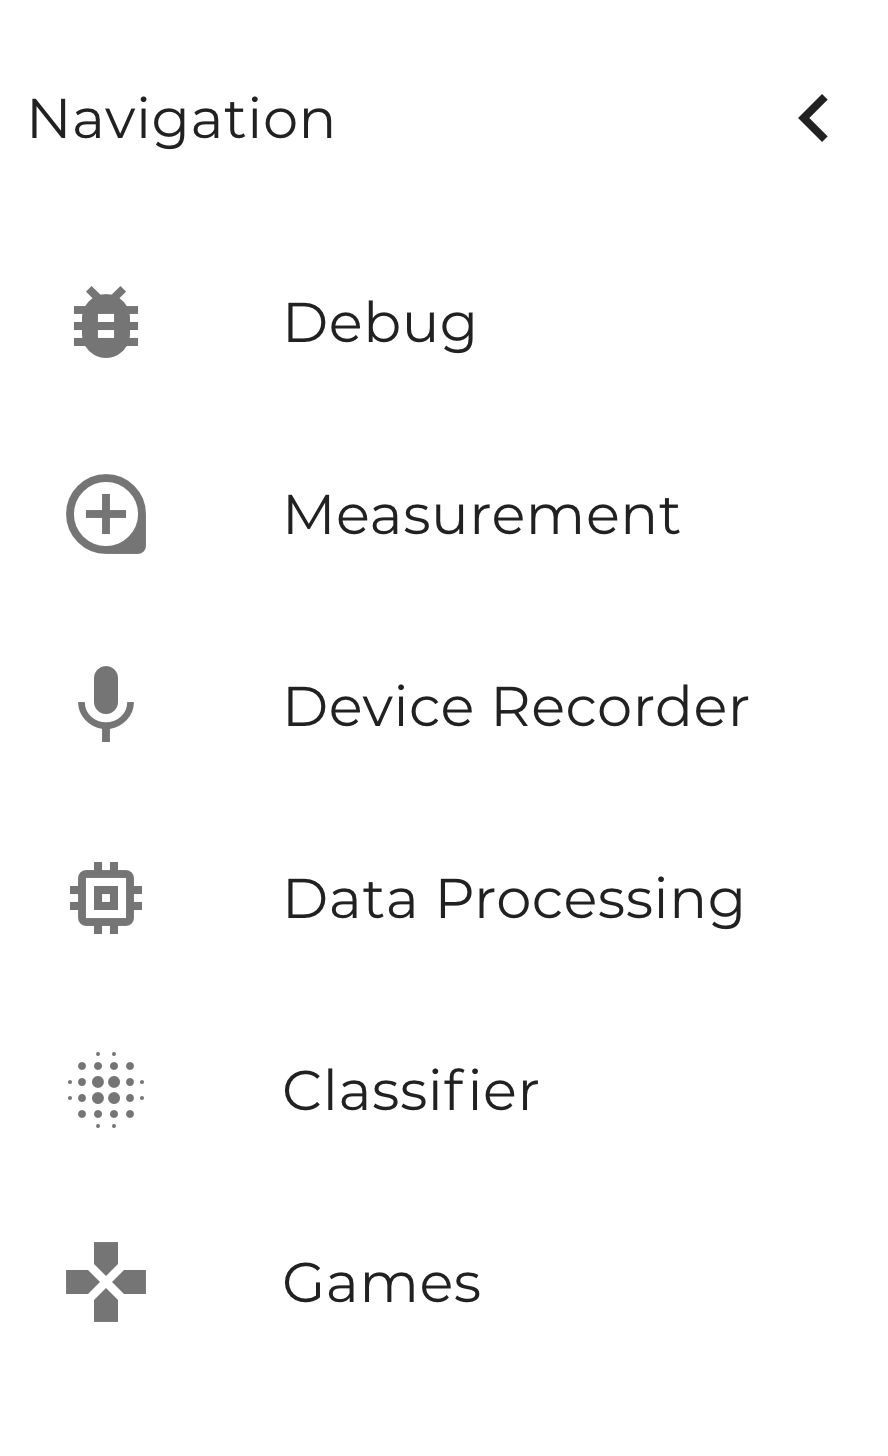
\includegraphics[width=6cm]{navigation}
    \caption{All Navigation Options of the Software}
    \label{fig:navigation}
\end{figure}
You can press the Button on the top left corner to get the Navigation Bar as shown in Figure \ref{fig:navigation}. From here, you can navigate to all available Subcomponents of the Software.

\subsection{Debug}
This is a section containing Information useful to Developers. You can look at the Data coming from the Device, or a graphical representation of your hand here. You probably won't need to spend too much time here though.

\subsection{Measurement}
Here, you can take the angular measurements between your Fingers, a piece of Information required by the Therapist. In order for the measurement to become more accurate, you can choose to average it over several milliseconds, by putting your desired value in the Input Box. On the left hand side, you will see your hand as the Computer sees it. Make sure it is fully visible and is displaying everything correctly. If something is wrong, and the measurement can't be taken, you will be notified of what you need to do in order to fix the problem on the right side of the screen.

\subsection{Device Recorder}
With this Component, you can record your Hand, and play that Data back to the Framework as if it was coming from the real device. As a User of the System, you probably won't ever need this, but this Component is useful for Developers. To start a new Recording, click the \texttt{+} Button. Now you can title your Recording. You also see a miniature Hand on the right side, if you have your hand above the sensor. Once you're ready, press the \texttt{Record} Button. A progress bar will begin to fill, indicating how much space is left for your recording, once it is full, or you press the \texttt{Save} Button, your recording is done. Now you can flip the Switch to activate it. It will then be propagated through the whole System in an endless loop.

If you want to save the Recordings for a later time, make sure the \texttt{Persist Recordings} Checkbox in the Settings Tab is checked.

\subsection{Data Processing}
If your Computer experiences performance issues while working with the System, you can attempt to alleviate this a bit here. Each of the Box shown here is representing a specific preprocessing step. For example, you can limit the framerate of the Device to a lower value such as \texttt{28 FPS} by turning on the \texttt{Limit FPS} Preprocessor. Your system has to do less that way, which will result in a better performance.

\subsection{Classifier}
Here, the Gesture you need to perform in order to control the Games is configured. Each Box represents one specific Gestures. Only one Box can be turned on at a time. Inside the Box, you will find a description of what to do in order to trigger the Gesture, and also some Input Boxes that allow the therapist to configure the Exercise to your needs. He or she might tell you which numbers you should put in here if you train from home.

\subsection{Games}
Finally, here you can choose and play any Game you like. If the Leap Motion Device is attached correctly to your computer, \textbf{and} you turned on a Gesture Classifier in the \texttt{Classifier} Tab, the Button \texttt{Play with Motion Tracking} will be green. Click on it to start the Game. In the game, you can hit \texttt{Space} to Pause or \texttt{Esc} to Quit if you feel tired. Good luck!

\chapter{Developer Manual}
Developers are advised to read through the main part of the paper in order to gain a general understanding on how the framework functions. Additionally, instructions on how to compile the project, and run the project in a development mode are given in the \texttt{README.me}, in the Source Code Repository (see Appendix \ref{app:code}). This Manual briefly gives practical advice on how to implement the System Interfaces, namely the \texttt{Preprocessing}, \texttt{Gesture Classification}, and \texttt{Game} Interfaces.
\section{Adding a Preprocessor}
As an example, let's add a Preprocessor for the Leap Motion Device that filters out frames where more than one hand is detected.
\subsection{Implement the Preprocessor}
This Preprocessor is specific to Leap Motion Device data, so be sure to put it into the \texttt{src/processing/leap} folder.
\begin{minted}{typescript}
// src/processing/leap/droptwohands.ts
export const DropTwoHandsId = "DropTwoHands";

export class DropTwoHandsPreProcessor
  implements Operator<GenericHandTrackingData, GenericHandTrackingData> {
  constructor() {}

  public call(
    subscriber: Subscriber<GenericHandTrackingData>,
    source: Observable<GenericHandTrackingData>
  ) {
    return source
      .pipe(
        // filter every frame where the hand
        // array is longer than 1.
        filter((value: LeapHandTrackingData) => value.data.hands.length > 1)
      )
      .subscribe(subscriber);
  }
}
\end{minted}

\subsection{Register the Preprocessor to the Framework}
in \texttt{src/processing/resolver.ts}, register your Preprocessor.
\begin{minted}{typescript}
// src/processing/resolver.ts
export const ResolverRegistry: {
  [_: string]: { new (...args: any[]): Operator<any, any> };
} = {
  [DropNFramesPreProcessorId]: DropNFramesOperator,
  [DestroyUselessFramesId]: DestroyUselessFramesOperator,
  [FPSThrottlerId]: FPSThrottler,
  // our new preprocessor
  [DropTwoHandsId]; DropTwoHandsPreProcessor
};
\end{minted}

\subsection{Add the new Preprocessor to the Vuex State}
To the \texttt{preprocessors.ts} state submodule, add a the state of the preprocessor, and implement the \texttt{constructConfig} method.
\begin{minted}{typescript}
// src/state/modules/preprocessors.ts
state: {
    preprocesors: {
        ...
        dropTwoHandsPreProcessor: {
            enabled: false,
            constructConfig: () => {
                identifier: DropTwoHandsId,
                // We don't need args for this
                args: []
            }
        }
        ...
    }
}
\end{minted}
\subsection{Add a Description to the Frontend}
Create a new Vue Component, containing an \texttt{md-card}, describing your Preprocessor. Import and integrate it in the \texttt{PreProcessing.vue} Frontend Component. If the switch is flipped by the User, call \texttt{modifyPreProcessor}, and commit a state mutation to set the \texttt{enabled} property of your preprocessor to \texttt{true}. Finally, call \texttt{preprocessorSelectionUpdated}. This will tell the Device Driver that the Preprocessors have changed, call the state function \text{constructConfig} internally, and construct your Preprocessor, supplying any arguments to the constructor in the order you specified in the \texttt{args} array.
Create a new C
\section{Adding a Classifier}
\section{Adding a Game}

\end{appendices}


%%%----------------------------------------------------------
\MakeBibliography                        				% references
%%%----------------------------------------------------------

%%% special page for checking print size --------------------
\include{back/printbox}

%%%----------------------------------------------------------
\end{document}
%%%----------------------------------------------------------